%!TEX program = xelatex
\documentclass[UTF8,zihao=5]{ctexart} %ctex包的article


\usepackage[hidelinks]{hyperref}%超链接,自动加到目录里面



\title{{\bfseries\rmfamily\Huge{高等计算流体力学\hspace{1em}\\第4次作业}}}
\author{周涵宇 2022310984}
\date{}

\usepackage[a4paper]{geometry}
\geometry{left=0.75in,right=0.75in,top=1in,bottom=1in}%纸张大小和页边距

\usepackage[
UseMSWordMultipleLineSpacing,
MSWordLineSpacingMultiple=1.5
]{zhlineskip}%office风格的行间距

\usepackage{fontspec}
\setmainfont{Times New Roman}
\setsansfont{Source Sans Pro}
\setmonofont{Latin Modern Mono}
\setCJKmainfont{SimSun}[AutoFakeBold=true]
% \setCJKmainfont{仿宋}[AutoFakeBold=true]
\setCJKsansfont{黑体}[AutoFakeBold=true]
\setCJKmonofont{DengXian}[AutoFakeBold=true]

\setCJKfamilyfont{kaiti}{楷体}
\newfontfamily\CM{Cambria Math}


% \usepackage{indentfirst} %不工作 怎样调整ctex的段首缩进大小呢

\usepackage{fancyhdr}
\pagestyle{fancy}
\lhead{}
\chead{}
\rhead{}
\lfoot{}
\cfoot{\thepage}
\rfoot{}
\renewcommand{\headrulewidth}{1pt} %改为0pt即可去掉页眉下面的横线
\renewcommand{\footrulewidth}{1pt} %改为0pt即可去掉页脚上面的横线
\setcounter{page}{1}


% \usepackage{bm}

\usepackage{amsmath,amsfonts}
\usepackage{array}
\usepackage{enumitem}
\usepackage{unicode-math}

% \usepackage{titlesec} % it subverts the ctex titles
\usepackage{titletoc}


% titles in toc:
\titlecontents{section}
              [2cm]
              {\sffamily\zihao{5}\mdseries}%
              {\contentslabel{3em}}%
              {}%
              {\titlerule*[0.5pc]{-}\contentspage\hspace*{1cm}}

\titlecontents{subsection}
              [3cm]
              {\rmfamily\mdseries\zihao{5}}%
              {\contentslabel{3em}}%
              {}%
              {\titlerule*[0.5pc]{-}\contentspage\hspace*{1cm}}

\titlecontents{subsubsection}
              [4cm]
              {\rmfamily\mdseries\zihao{5}}%
              {\contentslabel{3em}}%
              {}%
              {\titlerule*[0.5pc]{-}\contentspage\hspace*{1cm}}
\renewcommand*\contentsname{\hfill \sffamily\mdseries 目录 \hfill}

\ctexset{
    section={   
        % name={前面,后面},
        number={\arabic{section}.},
        format=\sffamily\raggedright\zihao{4}\mdseries,
        indent= {0em},
        aftername = \hspace{0.5em},
        beforeskip=1ex,
        afterskip=1ex
    },
    subsection={   
        % name={另一个前面,另一个后面},
        number={\arabic{section}.\arabic{subsection}.}, %如果只用一个数字而非1.1
        format=\rmfamily\raggedright\mdseries\zihao{5},%正体字体,不加粗,main字体,五号字
        indent = {2em}, %缩进
        aftername = \hspace{0.5em},
        beforeskip=1ex,
        afterskip=1ex
    },
    subsubsection={   
        % name={另一个前面,另一个后面},
        number={\arabic{section}.\arabic{subsection}.\arabic{subsubsection}.}, %默认的 1.1.1
        format=\rmfamily\raggedright\mdseries\zihao{5},%无衬线字体,加粗,sans字体,五号字
        indent = {2em}, %缩进
        aftername = \hspace{0.5em},  %名字和标题间插入字符(此处是空白)
        beforeskip=1ex, %空行
        afterskip=1ex
    }
}

\usepackage{float}
\usepackage{graphicx}
\usepackage{multirow}
\usepackage{multicol}
\usepackage{caption}
\usepackage{subcaption}


%part、section、subsection、subsubsection、paragraph、subparagraph
\newcommand{\bm}[1]{{\mathbf{#1}}}
\newcommand{\trans}[0]{^\mathrm{T}}
\newcommand{\tran}[1]{#1^\mathrm{T}}
\newcommand{\hermi}[0]{^\mathrm{H}}
\newcommand{\conj}[1]{\overline{#1}}
\newcommand*{\av}[1]{\left\langle{#1}\right\rangle}
\newcommand*{\avld}[1]{\frac{\overline{D}#1}{Dt}}
\newcommand*{\pd}[2]{\frac{\partial #1}{\partial #2}}
\newcommand*{\pdcd}[3]{\frac{\partial^2 #1}{\partial #2 \partial #3}}
\newcommand*{\inc}[0]{{\Delta}}

\newcommand*{\uu}[0]{\bm{u}}
\newcommand*{\vv}[0]{\bm{v}}
\newcommand*{\g}[0]{\bm{g}}
\newcommand*{\nb}[0]{{\nabla}}



\begin{document}

\maketitle

\section{动网格微分方程}

\newcommand*{\xxii}[0]{\symbf{\xi}}
\newcommand*{\xx}[0]{\symbf{x}}
\newcommand*{\U}[0]{\symbf{U}}
\newcommand*{\F}[0]{\symbf{F}}
\newcommand*{\vg}[0]{\symbf{v}_g}

本文中采用张量实体的时候,点或者不写明都是点积,$\otimes$是并矢,$\bm{T}$上标
是二阶张量的转置。

根据变换$(\xx,t)\leftrightarrow(\xxii,\tau)$,其中:
$$
    \pd{(\xx,t)}{(\xxii,\tau)}=\begin{bmatrix}
        \bm{J} & \vg \\
        0      & 1   \\
    \end{bmatrix}
$$
因此其逆为
$$
    \pd{(\xxii,\tau)}{(\xx,t)}=\begin{bmatrix}
        \bm{J}^{-1} & -\bm{J}^{-1}\vg \\
        0           & 1               \\
    \end{bmatrix}
$$
可得守恒律:
$$
    \pd{\bm{U}}{t}+\F\cdot\nb_{\xx}=0
$$
可以变换为(准守恒形式):

\begin{equation}
    \pd{\bm{U}}{\tau}+\F\cdot\nb_{\xxii}\bm{J^{-1}}=0
    \label{eq:p_conser}
\end{equation}


记Jacobian的行列式为$|\bm{J}|=J$,则有导数关系:$\pd{J}{\bm{J}}=J\bm{J^{-T}}$,
因此有(几何守恒关系):

\begin{equation}
    \nb_{\xxii}\cdot(J\bm{J^{-1}})=0,\ \
    \nb_{\xxii}\cdot(J\bm{J^{-1}}\vg)-\pd{J}{\tau}=0
    \label{eq:geom_conser}
\end{equation}

这样,方程两边同时乘$J$容易得到:
\begin{equation}
    \pd{J\U}{\tau}+
    [J\F\bm{J^{-T}} - \bm{U}\otimes(J\bm{J^{-1}}\vg)]\cdot\nb_{\xxii}
    \label{eq:conser}
\end{equation}


这就是运动曲线坐标的守恒型方程。注意本文的$J$是$L^3$量纲(假如参数坐标无量纲),
与论文中通常的记号是相反的。

考虑分量:
$$
    \bm{J^{-1}}\equiv\begin{bmatrix}
        \pd{\xi}{x}   & \pd{\xi}{y}   & \pd{\xi}{z}   \\
        \pd{\eta}{x}  & \pd{\eta}{y}  & \pd{\eta}{z}  \\
        \pd{\zeta}{x} & \pd{\zeta}{y} & \pd{\zeta}{z} \\
    \end{bmatrix}, \ \
    \bm{J^{-1}}\vg\equiv \begin{bmatrix}
        \pd{\xi}{t}   \\
        \pd{\eta}{t}  \\
        \pd{\zeta}{t} \\
    \end{bmatrix}
$$
记:
$$
    J\bm{J^{-1}}\equiv\begin{bmatrix}
        J\pd{\xi}{x}   & J\pd{\xi}{y}   & J\pd{\xi}{z}   \\
        J\pd{\eta}{x}  & J\pd{\eta}{y}  & J\pd{\eta}{z}  \\
        J\pd{\zeta}{x} & J\pd{\zeta}{y} & J\pd{\zeta}{z} \\
    \end{bmatrix}
    =
    \begin{bmatrix}
        \hat{\xi}_x   & \hat{\xi}_y   & \hat{\xi}_z   \\
        \hat{\eta}_x  & \hat{\eta}_y  & \hat{\eta}_z  \\
        \hat{\zeta}_x & \hat{\zeta}_y & \hat{\zeta}_z \\
    \end{bmatrix},\ \
    J\bm{J^{-1}}\vg\equiv \begin{bmatrix}
        J\pd{\xi}{t}   \\
        J\pd{\eta}{t}  \\
        J\pd{\zeta}{t} \\
    \end{bmatrix}=
    \begin{bmatrix}
        \hat{\xi}_t   \\
        \hat{\eta}_t  \\
        \hat{\zeta}_t \\
    \end{bmatrix}
$$

以无粘通量为例:
$$
    \F
    =
    \begin{bmatrix}
        \rho u        & \rho v        & \rho w        \\
        \rho uu + p   & \rho uv       & \rho uw       \\
        \rho vu       & \rho vv + p   & \rho vw       \\
        \rho wu       & \rho wv       & \rho ww + p   \\
        (\rho E + p)u & (\rho E + p)v & (\rho E + p)w \\
    \end{bmatrix}
$$

则可以化简为
$$
    J\F\bm{J^{-T}} - \bm{U}\otimes(J\bm{J^{-1}}\vg) = \hat{\F}
$$

其中曲线坐标的无粘通量为:

\begin{equation}
    \hat{\F}
    =
    \begin{bmatrix}
        \rho \hat{U}                        & \rho \hat{V}                         & \rho \hat{W}                          \\
        \rho u\hat{U} + \hat{\xi}_x p       & \rho u\hat{V} + \hat{\eta}_x p       & \rho u\hat{W} + \hat{\zeta}_x p       \\
        \rho v\hat{U} + \hat{\xi}_y p       & \rho v\hat{V} + \hat{\eta}_y p       & \rho v\hat{W} + \hat{\zeta}_y p       \\
        \rho w\hat{U} + \hat{\xi}_z p       & \rho w\hat{V} + \hat{\eta}_z p       & \rho w\hat{W} + \hat{\zeta}_z p       \\
        (\rho E + p)\hat{U} - \hat{\xi}_t p & (\rho E + p)\hat{V} - \hat{\eta}_t p & (\rho E + p)\hat{W} - \hat{\zeta}_t p \\
    \end{bmatrix}
    \label{eq:Fhat_inv}
\end{equation}

里面有曲线坐标对流速度:
$$
    \begin{aligned}
        \hat{U} = \hat{\xi}_t + \hat{\xi}_x u + \hat{\xi}_y v + \hat{\xi}_z w         \\
        \hat{V} = \hat{\eta}_t + \hat{\eta}_x u + \hat{\eta}_y v + \hat{\eta}_z w     \\
        \hat{W} = \hat{\zeta}_t + \hat{\zeta}_x u + \hat{\zeta}_y v + \hat{\zeta}_z w \\
    \end{aligned}
$$
守恒量中能量方程取$E$的方程。

这时,守恒型方程可以简写为:
$$
    \pd{J\U}{\tau}+
    \hat{\F}\cdot\nb_{\xxii}=0
$$

粘性通量可以进一步推导,但是基本关系满足\eqref{eq:conser}的结论。
根据\eqref{eq:Fhat_inv}的形式,取守恒量为均匀场,
通量偏导数为0的条件就是\eqref{eq:geom_conser}的几何守恒关系。
因此,在动曲线网格中若想满足均匀流保持条件,需要数值上满足\eqref{eq:geom_conser}。

\section{守恒差分}

在静止网格中,根据上一题,代入均匀场,对比方程\eqref{eq:p_conser}与\eqref{eq:conser},可发现
若采用守恒方程进行离散,则若要求时间导数是0,必须满足几何关系\eqref{eq:geom_conser}的第一部分(因为静止),
分量形式为:

\begin{equation}
    \begin{aligned}
        (\hat{\xi_x})\xi + (\hat{\eta_x})\eta + (\hat{\zeta_x })\zeta & = 0 \\
        (\hat{\xi_y})\xi + (\hat{\eta_y})\eta + (\hat{\zeta_y })\zeta & = 0 \\
        (\hat{\xi_z})\xi + (\hat{\eta_z})\eta + (\hat{\zeta_z })\zeta & = 0 \\
    \end{aligned}
    \label{eq:gc1}
\end{equation}

以上关系对于任何微分变换是精确成立的。

数值上,以上的最外层求导是参数坐标下的实际差分格式,
而内层的导数是通过$\bm{J}$的计算出来的,同时$\bm{J}$一般也是差分给出(也有可能是解析的),
其中的误差就可以导致以上关系不成立,因此有可能违反均匀流保持的条件。

以三维为例,直接计算时,
三维Jacobian矩阵的逆可以直接给出公式,因此展开后,\eqref{eq:gc1},
中第一个方程的实际计算过程是:
\begin{equation}
    (y_\eta z_\zeta)_\xi -
    (y_\zeta z_\eta)_\xi
    +
    (y_\zeta z_\xi)_\eta -
    (y_\xi z_\zeta)_\eta
    +
    (y_\xi z_\eta)_\zeta -
    (y_\eta z_\xi)_\zeta = 0
\end{equation}
以上括号内部的导数都是计算Metric的时候的差分格式,外部的导数是物理量的差分格式,
一般来说这是无法数值上保障为零的。

根据文献(R.Hixon, 2000),假设采用的外部差分格式具有交换性,即括号外部的混合偏导可以
交换次序,同时所有的偏导数,包括物理量的导数,都用这个差分格式计算:

\begin{equation}
    \begin{aligned}
        \hat{\xi}_x   & = (y_\eta z)_\zeta - (y_\zeta z)_\eta \\
        \hat{\xi}_y   & = (x_\zeta z)_\eta - (x_\eta z)_\zeta \\
        \hat{\xi}_z   & = (x_\eta y)_\zeta - (x_\zeta y)_\eta \\
        \hat{\eta}_x  & = (y_\zeta z)_\xi - (y_\xi z)_\zeta   \\
        \hat{\eta}_y  & = (x_\xi z)_\zeta - (x_\zeta z)_\xi   \\
        \hat{\eta}_z  & = (x_\zeta y)_\xi - (x_\xi y)_\zeta   \\
        \hat{\zeta}_x & = (y_\xi z)_\eta - (y_\eta z)_\xi     \\
        \hat{\zeta}_y & = (x_\eta z)_\xi - (x_\xi z)_\eta     \\
        \hat{\zeta}_z & = (x_\xi y)_\eta - (x_\eta y)_\xi     \\
    \end{aligned}
\end{equation}
上式中至少外部的偏导数是用和物理量相同的差分格式进行的。这个式子和
直接离散的过程数值上不等价,但是解析上是等价的。
那么第一个守恒律变成:
\begin{equation}
    (y_\eta z)_{\zeta\xi} -
    (y_\zeta z)_{\eta\xi}
    +
    (y_\zeta z)_{\xi\eta} -
    (y_\xi z)_{\zeta\eta}
    +
    (y_\xi z)_{\eta\zeta} -
    (y_\eta z)_{\xi\zeta} = 0
\end{equation}
括号外都是可交换的差分格式,因此其数值上可以保障为0。

当然,对于WENO等非线性差分格式,具体的导数计算还需要进一步讨论;
假如在网格上进行有限体积离散,则需要考虑半网格点上的导数计算和通量的等效性。

\section{差分离散稳定性}

这是对于一维线性对流扩散方程的离散,可看作对流项迎风二阶差分,扩散项中心格式外加显式欧拉时间推进。
设无限大计算域,则代入周期解:
$$
    u^n=\exp{(ikx)}
$$
则有:
$$
    \frac{u^{n+1} - \exp{(ikx)}}{\inc t}
    =-a \frac{3 - 4 \exp{(-ik\inc x)} + \exp{(-2ik\inc x)}}{2\inc x}\exp{(ikx)}
    +\nu \frac{\exp{(-ik\inc x)}-2+\exp{(ik\inc x)}}{\inc x^2}\exp{(ikx)}
$$
设$c=\frac{a\inc t}{\inc x},\sigma = \frac{\nu\inc t}{\inc x^2}, u^{n+1}=K\exp{(ikx)} $
则化为:
$$
    K
    =1-c\left(
    \frac{3}{2} - 2\exp(-ik\inc x) + \frac{1}{2}\exp(-2ik\inc x)
    \right)
    +\sigma\left(
    \exp(ik\inc x)+\exp(-ik\inc x)-2
    \right)
$$
记$k\inc x = \kappa $,则:
$$
    \Re(K) = 1+\left(2\,\cos\left(\kappa \right)-\frac{\cos\left(2\,\kappa \right)}{2}-\frac{3}{2}\right)\,c+\left(2\,\cos\left(\kappa \right)-2\right)\,\sigma
$$
$$
    \Im(K) = c\,\left(\frac{\sin\left(2\,\kappa \right)}{2}-2\,\sin\left(\kappa \right)\right)
$$
假如$c=0$,使得对于所有$\kappa$,$|K|<1$的条件是$\sigma < \frac{1}{2}$。
假如$\sigma = 0$, 对于所有$\kappa$,$|K|<1$是不可能存在的(总有很小的增长)。

为了直观分析其稳定性,给出数值结果,对于$c,\sigma$数值采样进行计算,
在$[0,1]\times[0,1]$考察$|K|$的大小,结果为:
\begin{figure}[H]
    \centering
    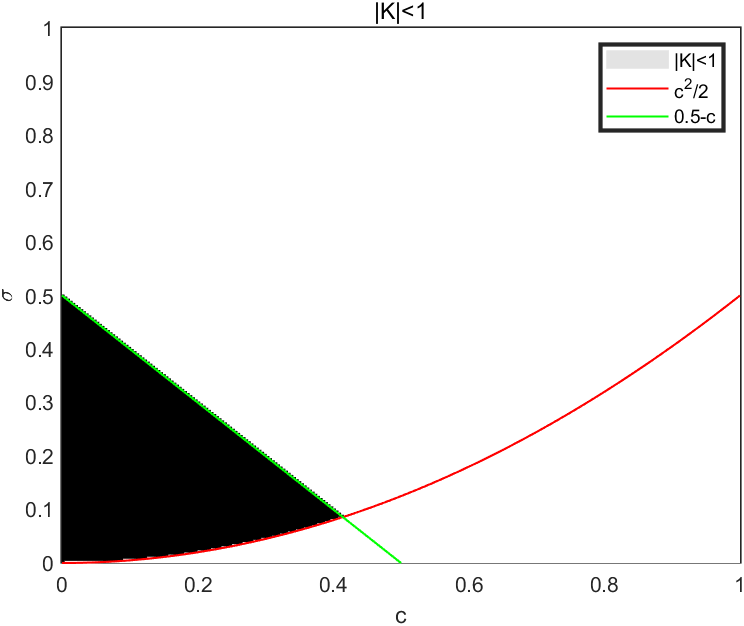
\includegraphics[width=8cm]{StableA.png}  %需调整
    \caption{$|K|$的大小区域,黑色区域为小于1}
    \label{fig:a}
\end{figure}

图中可见,在区域$\frac{c^2}{2}<\sigma<\frac{1}{2}-c$的区域为稳定的。
对于最小的$\sigma$,可见其正好与Warming-Beam格式的人工粘性部分大小相同。
根据以上结论,Warming-Beam的稳定要求为$0\leq c\leq\sqrt{2}-1$。






















% \section{SECTION 节}

% 一个

% \subsection{SUBSECTION 小节}

% 示例

% \subsubsection{SUBSUBSECTION 小节节}

% 字体字号临时调整:
% {
%    \sffamily\bfseries\zihao{3} 哈哈哈哈哈 abcde %三号 sans系列字体(一开始设置的) 加粗
%    %只对大括号范围内的后面的字有用,在标题、题注里面同样
% }
% { 
%    \CJKfamily{kaiti}\zihao{5}\itshape 哈哈哈哈哈 abcde%三号 kaiti(一开始设置的, 斜体(英文有变)
%    %只对大括号范围内的后面的字有用,在标题、题注里面同样
% }

% 一大堆一大堆一大堆一大堆一大堆一大堆一大堆一大堆一大堆一大堆
% 一大堆一大堆一大堆一大堆一大堆一大堆一大堆一大堆一大堆一大堆一大堆一大堆
% 一大堆一大堆一大堆一大堆一大堆一大堆一大堆一大堆一大堆一大堆一大堆一大堆
% 一大堆一大堆一大堆一大堆一大堆一大堆一大堆一大堆一大堆一大堆一大堆一大堆

% \begin{center}
%     居中的什么乱七八糟东西
% \end{center}


% 一个列表:
% \begin{itemize}
%     \item asef
%     \item[\%] asdf
%     \item[\#] aaa
% \end{itemize}

% 一个有序列表:
% \begin{enumerate}
%     \item asef
%     \item[\%\%] asdf
%     \item aaa
% \end{enumerate}

% 一个嵌套列表,考虑缩进:
% \begin{enumerate}[itemindent=2em] %缩进
%     \item asef \par asaf 东西东西东西东西东西东西东西东西东西东西东西东西东西东西东西东西东西东西东西东西东西东西东西东西,
%           F不是不是不是不是不是不是不是不是不是不是不是不是不是不是不是
%           \begin{itemize}[itemindent=2em]  %缩进
%               \item lalala
%               \item mamama
%           \end{itemize}
%     \item asdf
%     \item aaa
% \end{enumerate}

% \section{SECTION}

% 图片排版:

% \begin{figure}[H]
%     \begin{minipage}[c]{0.45\linewidth}  %需调整
%         \centering
%         \includegraphics[width=8cm]{RAM_O2_4660.png}  %需调整
%         \caption{第一个图}
%         \label{fig:a}
%     \end{minipage}
%     \hfill %弹性长度
%     \begin{minipage}[c]{0.45\linewidth}  %需调整
%         \centering
%         \includegraphics[width=8cm]{RAM_O4_4660.png}  %需调整
%         \caption{第二个图}
%         \label{fig:b}
%     \end{minipage}
% \end{figure}

% figure的选项为“htbp”时,会自动浮动,是“H”则和文字顺序严格一些。

% \begin{figure}[H]
%     \begin{minipage}[c]{0.45\linewidth}  %需调整
%         \centering
%         \includegraphics[width=8cm]{RAM_O2_4660.png}  %需调整
%         \label{fig:x}
%     \end{minipage}
%     \hfill %弹性长度
%     \begin{minipage}[c]{0.45\linewidth}  %需调整
%         \centering
%         \includegraphics[width=8cm]{RAM_O4_4660.png}  %需调整
%         \label{fig:y}
%     \end{minipage}
%     \caption{第三个图}
% \end{figure}

% \begin{figure}[H]
%     \centering
%     \includegraphics[width=8cm]{RAM_O4_4660.png}  %需调整
%     \label{fig:c}
%     \caption{第四个图}
% \end{figure}



% \subsection{SUBSECTION}

% 关于怎么搞表格:

% \begin{table*}[htbp]
%     \footnotesize
%     \begin{center}
%         \caption{一端力矩载荷下的结果\fontsize{0pt}{2em}} %需要学习统一设置;0代表不变?
%         \label{表2}
%         \begin{tabular}{|c|c|c|c|c|c|c|}
%             \hline
%             节点数                              & 积分方案              & 单元数                & $h=1m$                & $h=0.1m$              & $h=0.05m$             & $h=0.01m$             \\
%             \hline
%             \multirow{6}{*}{2}                  & \multirow{3}{*}{精确} & 1                     & 4.235294117647059E-08 & 1.406250000000000E-06 & 2.862823061630218E-06 & 1.439654482924097E-05 \\
%             \cline{3-7}
%                                                 &                       & 10                    & 5.975103734439814E-08 & 4.235294117646719E-05 & 1.800000000000410E-04 & 1.406249999999849E-03 \\
%             \cline{3-7}
%                                                 &                       &
%             10000                               & 5.999999915514277E-08 & 5.999996622448291E-05 & 4.799989509752562E-04 & 5.999793702477535E-02                                                 \\
%             \cline{2-7}
%                                                 & \multirow{3}{*}{减缩} & 1                     & 6.000000000000001E-08 & 5.999999999999972E-05 & 4.799999999999911E-04 & 6.000000000003492E-02 \\
%             \cline{3-7}
%                                                 &                       & 10                    & 6.000000000000071E-08 & 5.999999999999142E-05 & 4.799999999995399E-04 & 5.999999999903294E-02 \\
%             \cline{3-7}
%                                                 &                       & 10000                 & 6.000000112649221E-08 & 5.999999234537814E-05 & 4.799997501925065E-04 & 6.000037607984510E-02 \\
%             \hline

%             \multirow{6}{*}{3}                  & \multirow{3}{*}{精确} & 1                     & 6.000000000000003E-08 & 6.000000000000202E-05 & 4.800000000000831E-04 & 6.000000000056749E-02 \\
%             \cline{3-7}
%                                                 &                       & 10                    & 5.999999999999932E-08 & 6.000000000004190E-05 & 4.800000000000206E-04 & 6.000000001613761E-02 \\
%             \cline{3-7}
%                                                 &                       & 10000                 & 6.000000013769874E-08 & 5.999989495410481E-05 & 4.799942099727246E-04 & 6.000263852944890E-02 \\
%             \cline{2-7}
%                                                 & \multirow{3}{*}{减缩} & 1                     & 6.000000000000002E-08 & 6.000000000000267E-05 & 4.800000000000754E-04 & 5.999999999989982E-02 \\
%             \cline{3-7}
%                                                 &                       & 10                    & 5.999999999999899E-08 & 5.999999999987338E-05 & 4.799999999947916E-04 & 5.999999998625345E-02 \\
%             \cline{3-7}
%                                                 &                       & 10000                 & 5.999999728157785E-08 & 5.999994914321980E-05 & 4.800008377474699E-04 & 5.999472246346305E-02 \\
%             \hline

%             \multicolumn{3}{|c|}{欧拉-伯努利解} & 6.000000000000000E-08 & 6.000000000000000E-05 & 4.800000000000000E-04 & 6.000000000000000E-02                                                 \\
%             \hline
%         \end{tabular}
%     \end{center}
% \end{table*}

% 多行、多列表格的示例,基本思想是,多列的那个东西放在多列的最上面一格,下面的行要用\&来空开,也就是\&的数目
% 和普通表格一样,是列数减一;
% 多列的部分的话,就是每行内的操作,相应的\&就少了,见最后一行。

% tabular的“|c|c|c|c|c|c|c|”,意思是,竖线-居中-竖线-居中-竖线……,可以选择省略一些竖线;
% 每行之间的hline,代表贯通的横线,cline是有范围的横线。

% \subsubsection{SUBSUBSECTION}

% newcommand可以用来定义新指令,似乎基本上就是字符串替换……不太懂,总之在公式里面可以用,
% 外面也经常用。






% 公式这么写:
% \begin{equation}
%     \begin{aligned}
%         \frac{aa(x^1+x^2)}{\sqrt{x^1x^2}}
%         \nabla\times\uu
%         = & u_{j;m}\g^m\times\g^j
%         =u_{j;m}\epsilon^{mjk}\g_k
%         =u_{j,m}\epsilon^{mjk}\g_k                           \\
%         = & \frac{1}{\sqrt{g}}\left|
%         \begin{matrix}
%             \g_1       & \g_2       & \g_3       \\
%             \partial_1 & \partial_2 & \partial_3 \\
%             u_1        & u_2        & u_3
%         \end{matrix}
%         \right|
%         =\frac{\sqrt{x^1x^2}}{aa(x^1+x^2)}
%         \left|
%         \begin{matrix}
%             \g_1                        & \g_2                        & \g_3       \\
%             \partial_1                  & \partial_2                  & \partial_3 \\
%             u^1\frac{a^2(x^1+x^2)}{x^1} & u^2\frac{a^2(x^1+x^2)}{x^2} & u^3
%         \end{matrix}
%         \right|                                              \\
%         = & \frac{\sqrt{x^1x^2}}{aa(x^1+x^2)}
%         [[\g_1\,\g_2\,\g_3]]
%         diag\left(
%         u^3_{,2}-u^2_{,3}\frac{a^2(x^1+x^2)}{x^2},\,
%         u^1_{,3}\frac{a^2(x^1+x^2)}{x^1}-u^3_{,1},\, \right. \\
%           & \left.
%         u^2_{,1}\frac{a^2(x^1+x^2)}{x^2}+u^2\frac{a^2}{x^2}
%         -
%         u^1_{,2}\frac{a^2(x^1+x^2)}{x^1}-u^1\frac{a^2}{x^1}
%         \right)                                              \\
%         = & \frac{\sqrt{x^1x^2}}{aa(x^1+x^2)}
%         [[\bm{e}_1\,\bm{e}_2\,\bm{e}_3]]
%         \left[\begin{array}{ccc} a & -a & 0\\ \frac{a\,x^{2}}{\sqrt{x^{1}\,x^{2}}} & \frac{a\,x^{1}}{\sqrt{x^{1}\,x^{2}}} & 0\\ 0 & 0 & 1 \end{array}\right]              \\
%           & diag\left(
%         u^3_{,2}-u^2_{,3}\frac{a^2(x^1+x^2)}{x^2},\,
%         u^1_{,3}\frac{a^2(x^1+x^2)}{x^1}-u^3_{,1},\, \right. \\
%           & \left.
%         u^2_{,1}\frac{a^2(x^1+x^2)}{x^2}+u^2\frac{a^2}{x^2}
%         -
%         u^1_{,2}\frac{a^2(x^1+x^2)}{x^1}-u^1\frac{a^2}{x^1}
%         \right)
%     \end{aligned}
%     \label{eq:curlu}
% \end{equation}

% 如果不想带编号的公式(或者图表),用 equation* 这种环境。

% 引用,如果是引用的图表,就用表\ref{表2},图\ref{fig:a}这种,代码里是用label定义的标签来引用,
% 编号是自动生成的。公式引用一般写成:\eqref{eq:curlu}。目前这些引用自动会有超链接,反正有那个包自动
% 好像就会有……呜呜呜也不知道是怎么做到的,先这么用吧。

% \paragraph{PARA}

% 引用文献用\\cite这些,要用bibtex,暂时不做。

% \subparagraph{SUBPARA}

\end{document}